\section{Application aux données simulées}
\subsection{Choix de K et coupures}
Le coude du critère $C$ de Fisher conduit à $K=4$ (figure~\ref{fig:coude})
\cite{same}. Les valeurs à $K=3,4,5$ sont
$462{,}01$, $300{,}60$, $292{,}37$ : le gain passe de $161{,}42$ à $8{,}22$
(de $34{,}9\,\%$ à $2{,}7\,\%$).
Minimiser directement $C$ sur $K$ serait inadapté, car $K=n$ donne zéro.

\begin{figure}[H]
\centering
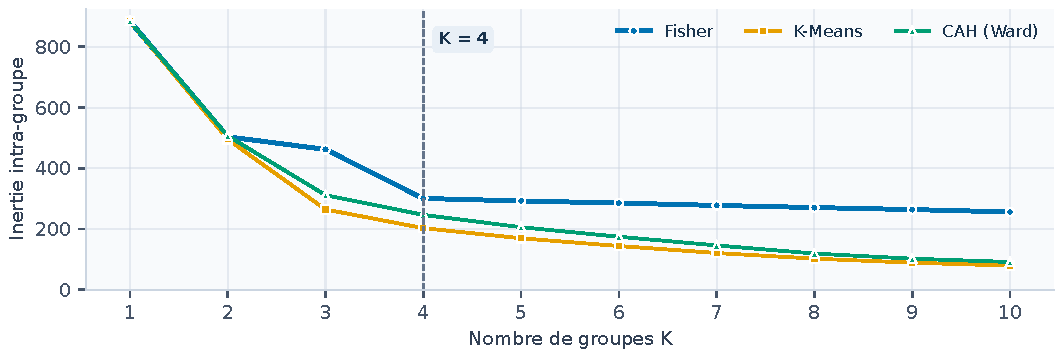
\includegraphics[width=0.94\linewidth,height=4.7cm,keepaspectratio]{simulation_coude.pdf}
\caption[Simulation : inertie et choix du nombre de segments]{Inerties sur \file{sequencesimu}. Le trait vertical indique $K=4$ ;
les K-means utilisent 20 départs, graine 42.}
\label{fig:coude}
\end{figure}
Les coupures Python sont $[50,80,130]$, soit $[51,81,131]$ en numérotation à partir de 1.
Les segments $1$--$50$, $51$--$80$, $81$--$130$, $131$--$160$ ont pour
effectifs $[50,30,50,30]$.

\subsection{Comparaison des partitions}
\begin{figure}[H]
\centering
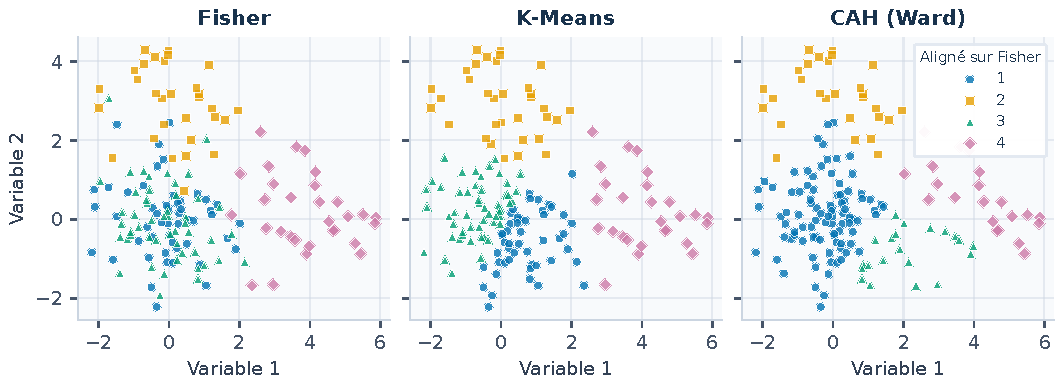
\includegraphics[width=0.98\linewidth,height=4.8cm,keepaspectratio]{simulation_espace.pdf}
\caption[Simulation : partitions dans l'espace]{Partitions dans le plan des deux variables. Les couleurs sont alignées
sur Fisher : les segments 1 et 3 se recouvrent spatialement.}
\label{fig:simuespace}
\end{figure}

\begin{figure}[H]
\centering
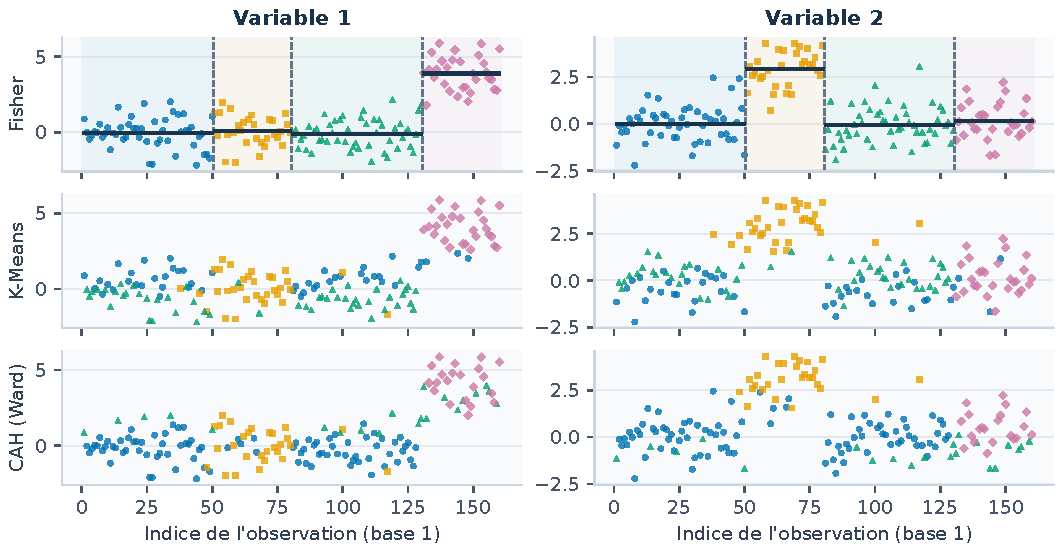
\includegraphics[width=0.98\linewidth,height=7.4cm,keepaspectratio]{simulation_temps.pdf}
\caption[Simulation : partitions selon l'ordre des observations]{Partitions à $K=4$ selon l'ordre des observations ; pointillés :
coupures Fisher ; traits horizontaux : moyennes ajustées par segment.
Les couleurs sont alignées sur les segments Fisher.}
\label{fig:simutemps}
\end{figure}
\begin{table}[H]
\centering\small
\begin{tabular}{lrr}
\toprule
Méthode & Inertie & Changements voisins \\
\midrule
Fisher & 300{,}60 & 3 \\
K-Means & 202{,}89 & 75 \\
CAH (Ward) & 246{,}58 & 45 \\
\bottomrule
\end{tabular}

\caption[Simulation : inertie et changements de label]{Inertie et nombre de changements de label entre observations voisines.}
\label{tab:simucomparaison}
\end{table}

Le recouvrement des segments 1 et 3 (figure~\ref{fig:simuespace}) explique
que les méthodes non contraintes regroupent des points de périodes différentes.
Leur inertie plus faible traduit une meilleure compacité spatiale, mais les
alternances de labels révèlent une fragmentation temporelle. Fisher préserve
la cohérence des régimes successifs. Sans étiquettes de référence, cette
comparaison ne mesure toutefois pas l'exactitude des partitions.
